\documentclass{mythesis}

\usetikzlibrary{patterns}

\usepackage{titling}

\title{Inpainting mit Eulers Elastica}
\author{Stephan Hilb}


%\DeclareDocumentCommand{\thesection}{}{\arabic{section}}
%\DeclareDocumentCommand{\thesubsection}{}{\thesection.\arabic{subsection}}

% "such that"
\DeclareDocumentCommand{\st}{}{\mathbin{|}}

\DeclareDocumentCommand{\Edat}{}{E_{\mathrm{dat}}}
\DeclareDocumentCommand{\Eimg}{}{E_{\mathrm{img}}}

\DeclareDocumentCommand{\BV}{}{\mathord{\mathrm{BV}}}


\tikzset{missing/.style={dashed,pattern=checkerboard,pattern color=red!15}}

\colorlet{fg}{black}
\colorlet{bg}{white}


\begin{document}

%\usepackage{titling}

\begin{titlepage}
  \begin{center}
    ~\par\vspace{4em}
    {
      \fontsize { 16pt } { 16pt } \selectfont
      Masterarbeit
    }
    \par\vspace{3em}
    {
      \fontsize { 24pt } { 24pt } \selectfont \sffamily \bfseries
      \thetitle
    }
    \par\vspace{3em}
    {
      \fontsize { 16pt } { 16pt } \selectfont \scshape
      \theauthor
    }
    \par\vspace{1.5em}
    {
      \fontsize { 14pt } { 14pt } \selectfont %\scshape
      \today
    }
    \par\vspace{4.5em}
    {
    }
    \par\vspace{8em}
    {
      \fontsize { 14pt } { 14pt } \selectfont \scshape
      Universität Stuttgart
    }
    \par\vspace{1em}
    {
      \fontsize { 14pt } { 14pt } \selectfont %\scshape
      Institut für Angewandte Analysis und Numerische Simulation
    }
    \par\vspace{1em}
    {
      \fontsize { 14pt } { 14pt } \selectfont %\scshape
      Betreuer:
      Dr. Claus J. Heine,
      Dr. Andreas Langer
    }
  \end{center}
\end{titlepage}

\chapter*{Zusammenfassung}

Die Zielsetzung, fehlende Teile eines Bildes zu rekonstruieren – auch „Inpainting“ genannt – lässt sich als Minimierung eines
Funktionals für das Gesamtbild modellieren, bestimmt durch ein Datenmodell, das die Übereinstimmung mit dem ursprünglichen Bild auf dem bekannten Gebiet kontrolliert, und einem Bildmodell, welches maßgebend für die Güte der Rekonstruktion ist.

Das Euler Elastica Bildmodell, welches die Niveaulinien eines Bildes nach dem Vorbild elastischer Stäbe modelliert, bietet ein vielversprechendes Bildmodell und kommt in dieser Arbeit zum Einsatz.
Für die numerische Minimierung wird eine bekannte “alternating direction“ Augmented Lagrange Methode angewandt und die entstehenden Teilprobleme erstmalig im Kontext der Finiten Elemente gelöst.


{
  \let\clearpage\relax
  \tableofcontents
  %\addtocentrydefault{chapter}{}{Inhaltsverzeichnis}
}
%\tableofcontents



\chapter{Einführung}

%
%\begin{itemize}
%    \item
%	Lösungsansätze für das EE inpainting model in der Literatur
%\end{itemize}
%
%Mit Blick auf \ref{fig:setting} führen wir zunächst Begrifflichkeiten ein.

\begin{definition} \label{def:image}
    Ein \emphdef{Bild} ist eine Abbildung $u: \Omega \to F$, wobei $\Omega \subset \R^d$
    \emphdef{Trägermenge} genannt wird und $F$ \emphdef{Farbraum}.
    Für einen festen Farbraum $F$ sei $I_X$ die Menge der Bilder mit Trägermenge $X$.
    \begin{note}
	Wir betrachten im weiteren Verlauf Graustufenbilder und setzen daher stets $F := [0,1]$ (mit der
	Interpretation: $0$ entspricht „schwarz“ und $1$ „weiß“).
    \end{note}
\end{definition}

Wann immer man Strukturen oder geometrische Eigenschaften in solchen Bildern untersuchen möchte, ist man dazu geneigt diese Definition einzuschränken (indem man z.B. eine Form von Differenzierbarkeit fordert).
Obwohl dies oft im Widerspruch zu den üblichen Eigenschaften von Bildern steht (z.B. Unstetigkeiten an Kanten und Konturen), werden wir dies später an den entsprechenden Stellen tun.

\begin{figure}[ht]
    \centering
    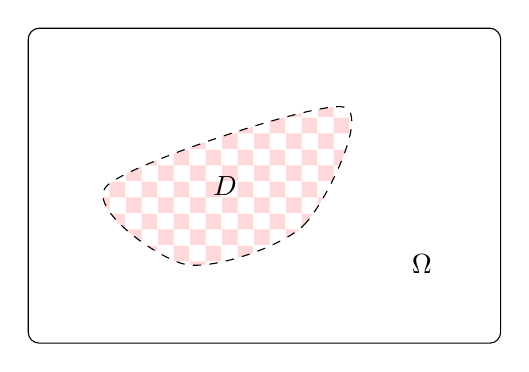
\begin{tikzpicture}
	\draw[rounded corners] (0,0) rectangle (6,4);
	\draw (5,1) node {$\Omega$};
	\draw[missing] plot[smooth cycle] coordinates {(2,1) (3.5,1.5) (4,3) (1,2)};
	\draw (2.5,2) node {$D$};
    \end{tikzpicture}
    \caption{Typische Inpainting-Situation}
    \label{fig:inpainting_setting}
\end{figure}

Beim Inpainten gehen wir von einem gegebenen Bild $u^0: \Omega \setminus D \to [0,1]$ und einem \emphdef{Inpainting-Bereich}
$D \subset \Omega$ aus (siehe \ref{fig:inpainting_setting}. Ziel ist nun eine Rekonstruktion $u: \Omega \to [0,1]$, die optisch „möglichst gut zu $u^0$ passt“.

Wir werden „möglichst gut“ durch die Minimierung eines Energiefunktionals $E[u]$ bestehend aus einem Datenmodell (engl. “data model”) und einem Bildmodell (engl. “image prior model”) ersetzen.
Der Bayes'sche Ansatz liefert hierfür eine schmackhafte Motivation.


\section{Das Bayes'sche Prinzip}

Es seien hier $I_\Omega$, $I_{\Omega \setminus D}$ endlich.
Dies ist beispielsweise der Fall, wenn $\Omega \subset \Z^d$ beschränkt und $F$ endlich ist, was bei praktisch allen digitalen Bildern zwingend ist.

\begin{samepage}
Geht man davon aus, dass $u^0$ zu einem ursprünglichen, vollständigen Bild $u$ gehört, so lässt sich die Entstehung von $u^0$ als Zufallsexperiment in zwei Schritten modellieren:
\begin{enumerate}
    \item
	Auftreten von $u$ als Bild im (diskreten) Wahrscheinlichkeitsraum $(I_\Omega, 2^{I_\Omega}, P_{\mathrm{img}})$, \nopagebreak
    \item
        Zustandekommen von $u^0$ als Beobachtung von $u|_{\Omega \setminus D}$ in $(I_{\Omega \setminus D}, 2^{I_{\Omega \setminus D}}, P_{\mathrm{dat},u})$.
\end{enumerate}
\end{samepage}
Wir betrachten dazu den diskreten Wahrscheinlichkeitsraum $\scr P := (I_\Omega \times I_{\Omega\setminus D}, 2^{I_\Omega \times I_{\Omega\setminus D}}, P)$ mit der sogenannten A-Posteriori-Wahrscheinlichkeitsverteilung
\begin{math}
    P(u, u^0) := P_{\mathrm{img}}(u) \cdot P_{\mathrm{dat},u^0}(u)
\end{math}
In diesem Raum besitzt $P_{\mathrm{dat},u^0}(u)$ die gewünschte Interpretation als bedingte Wahrscheinlichkeit $P(u^0|u)$:
\begin{math}
    P(u) &= P_{\mathrm{img}}(u), \\
    P(u^0|u) &= \frac{P(u, u^0)}{P(u)} = P_{\mathrm{dat},u^0}(u),
\end{math}
wobei wir $u$ und $u^0$ mit $\Set{u} \times I_{\Omega \setminus D}$, bzw. $I_\Omega \times \Set{u_0}$ identifizieren.
Dieser Raum erlaubt uns die Berechnung der bedingten Wahrscheinlichkeit
\begin{math}
    P(u|u^0) &= \frac{P(u, u^0)}{P(u^0)}
    = \frac{P(u^0|u) \cdot P(u)}{P(u^0)}.
\end{math}
Dieser einfache Zusammenhang zwischen den bedingten Wahrscheinlichkeiten ist auch als \emph{Satz von Bayes} bekannt.

Beim Inpainten ist $P(u^0)$ ist konstant und $P(u|u^0)$ die Wahrscheinlichkeit, dass $u$ die korrekte Rekonstruktion von $u^0$ ist, also maximieren wir
\begin{math}
    P(u|u^0) = \const \cdot P_{\mathrm{dat},u^0}(u) \cdot P_{\mathrm{img}}(u).
\end{math}
Wir können nun auf beiden Seiten $-\log(\argdot)$ anwenden und ein äquivalentes, aber durchaus handlicheres Problem in Energie-Form betrachten.

Für gegebenes $u^0$, $D$ minimieren wir also die Summe aus Datenterm und Bildterm (die additive Konstante ist für das Minimieren irrelevant)
\begin{math}
    E[u] = \Edat[u] + \Eimg[u].
\end{math}
Die Wahlen von $\Edat[u]$ und $\Eimg[u]$, welche den Wahrscheinlichkeitsverteilungen in unserem zweistufigen Zufallsmodell entsprechen, sind durch das Datenmodell, bzw. das Bildmodell festgelegt.


\section{Das Datenmodell}

Naheliegend ist der Gedanke, als Datenmodell lediglich $u|_{\Omega \setminus D} = u^0|_{\Omega \setminus D}$ zu fordern.
Damit würden feste Randbedingungen für das Minimieren auf $D$ vorgegeben werden.
In der Praxis sind Bilder jedoch meist mit Rauschen, Unschärfe oder anderen Artefakten versetzt, sei es aufgrund technischer Aufnahmebedingungen, natürlichen Zerfalls, digitaler Kompressionsartefakte oder aus anderen Gründen.
Das Datenmodell erlaubt es zu definieren, auf welche Weise $u|_{\Omega \setminus D}$ beim Inpainten an das vorliegende Bild $u^0$ angepasst werden soll und ermöglicht es solche Verunreinigungen auszugleichen.

Wir nutzen den bekannten Datenterm aus \cite{rudin1992nonlinear}, welcher die quadrierte $L^2$-Norm verwendet:
\begin{math}
    \Edat[u] = \frac{\eta}{2} \int_{\Omega \setminus D} |u - u^0|^2,
\end{math}
wobei $\eta \in \R_{> 0}$ die spätere Gewichtung des Datenterms zum Bildterm kontrolliert.

Es ist bekannt \cite[§4.5]{chan2005image}, dass dieser Datenterm gut geeignet ist, wenn das Orginalbild mit Gaus'schem Rauschen versetzt ist, modelliert als $u^0 = u|_{\Omega \setminus D} + \eta$.
Für Schwarz/Weiß Rauschen (auch “salt-and-pepper noise” oder “impulse noise” gennant) ist die Wahl einer $L^1$-Norm zu bevorzugen, wie in \cite{nikolova2004variational} gezeigt.

Denkbar wären auch Datenmodelle wie $u^0 = K[u|_{\Omega\setminus D}] + \epsilon$ für einen Glättungsoperator $K$.
Solche Modelle würden es erlauben, Unschärfe zu reduzieren, siehe z.B. \cite{rudin1994total}.


\section{Das Bildmodell}

Da der Datenterm sich auf $\Omega \setminus D$ beschränkt hat, trägt das Bildmodell die Hauptrolle bei der eigentlichen Bildrekonstruktion innerhalb von $D$.
Man beachte, dass das Bildmodell unabhängig von $D$ ist (man erinnere sich an das Bayes-Prinzip) und auch für $D = \emptyset$ (z.B. Denoising) die Rekonstruktion des ursprünglichen Bildes verbessern kann.
In der Literatur zum Denoising wird $\Eimg[u]$ daher auch als “regularization term” bezeichnet.

\begin{figure}[ht]
    \begin{subfigure}[b]{0.33\textwidth}
	\centering
        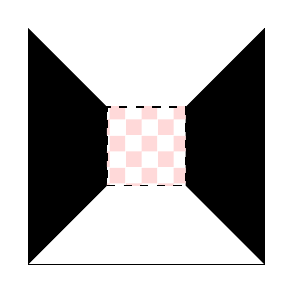
\begin{tikzpicture}
	    \draw[clip] (0,0) rectangle (3,3);
	    \fill[bg] (0,0) rectangle (3,3);
	    \fill[fg] (0,0) -- (1,1) -- (1,2) -- (0,3) -- cycle;
	    \fill[fg] (3,0) -- (3,3) -- (2,2) -- (2,1) -- cycle;
	    \draw[missing] (1,1) -- (2,1) -- (2,2) -- (1,2) -- cycle;
        \end{tikzpicture}
    \end{subfigure}%
    \begin{subfigure}[b]{0.33\textwidth}
	\centering
        
\begin{tikzpicture}
	    \draw[clip] (0,0) rectangle (3,3);
	    \fill[fg] (0,0) rectangle (3,3);
	    \fill[bg] (0,0) -- (3,0) -- (2,1) -- (1,1) -- cycle;
	    \fill[bg] (0,3) -- (1,2) -- (2,2) -- (3,3) -- cycle;
        \end{tikzpicture}
    \end{subfigure}%
    \begin{subfigure}[b]{0.33\textwidth}
	\centering
        
\begin{tikzpicture}
	    \draw[clip] (0,0) rectangle (3,3);
	    \fill[bg] (0,0) rectangle (3,3);
	    \fill[fg] (0,0) -- (1,1) -- (1,2) -- (0,3) -- cycle;
	    \fill[fg] (3,0) -- (3,3) -- (2,2) -- (2,1) -- cycle;
        \end{tikzpicture}
    \end{subfigure}
    \caption{Bewertungsschwierigkeiten: welches der beiden vollständigen Bildern ist wahrscheinlicher?}
    \label{fig:inpainting_non_unique}
\end{figure}

Zunächst macht man sich schnell anhand von einfachen Beispielen klar, dass die Wahl eines guten Bildmodells keineswegs einfach oder eindeutig ist, da die Bildbewertung oft von der menschlichen Interpretation abhängt.
Welche der beiden vollständigen Bilder aus Abbildung \ref{fig:inpainting_non_unique} ein Betrachter eher für richtig hält, hängt davon ab, ob er Hell oder Dunkel für vordergründiger hält.

\begin{figure}[ht]
    \begin{subfigure}[b]{0.33\textwidth}
	\centering
        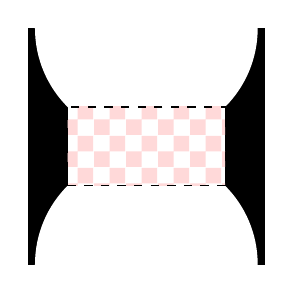
\begin{tikzpicture}
	    \draw[clip] (0,0) rectangle (3,3);
	    \fill[fg] (0,0) rectangle (3,3);
	    \fill[bg] (1.5,3) circle[radius=1.41421];
	    \fill[bg] (1.5,0) circle[radius=1.41421];
	    \fill[bg] (0.5,1) -- (2.5,1) -- (2.5,2) -- (0.5,2) -- cycle;
	    \draw[missing] (0.5,1) -- (2.5,1) -- (2.5,2) -- (0.5,2) -- cycle;
        \end{tikzpicture}
    \end{subfigure}%
    \begin{subfigure}[b]{0.33\textwidth}
	\centering
        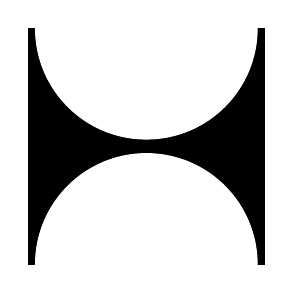
\begin{tikzpicture}
	    \draw[clip] (0,0) rectangle (3,3);
	    \fill[fg] (0,0) rectangle (3,3);
	    \fill[bg] (1.5,3) circle[radius=1.41421];
	    \fill[bg] (1.5,0) circle[radius=1.41421];
        \end{tikzpicture}
    \end{subfigure}%
    \begin{subfigure}[b]{0.33\textwidth}
	\centering
        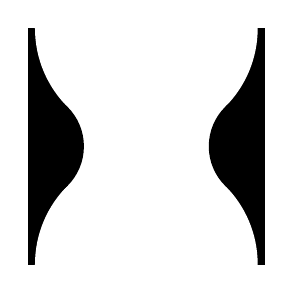
\begin{tikzpicture}
	    \draw[clip] (0,0) rectangle (3,3);
	    \fill[fg] (0,0) rectangle (3,3);
	    \fill[bg] (1.5,3) circle[radius=1.41421];
	    \fill[bg] (1.5,0) circle[radius=1.41421];
	    \fill[bg] (0.5,1) -- (2.5,1) -- (2.5,2) -- (0.5,2) -- cycle;
	    \fill[fg] (0,1.5) circle[radius=0.70710];
	    \fill[fg] (3,1.5) circle[radius=0.70710];
        \end{tikzpicture}
    \end{subfigure}
    \caption{Kurze Niveaulinien (rechts) werden bevorzugt}
    \label{fig:inpainting_prefer_short}
\end{figure}

%\begin{figure}[ht]
%    \begin{subfigure}[b]{0.33\textwidth}
%	\centering
%        \begin{tikzpicture}
%	    \draw[clip] (0,0) rectangle (3,3);
%	    \fill[fg] (0,0) rectangle (3,3);
%	    \fill[bg] (1.5,3) circle[radius=1.11803];
%	    \fill[bg] (1.5,0) circle[radius=1.11803];
%	    \fill[bg] (1,1) -- (2,1) -- (2,2) -- (1,2) -- cycle;
%	    \draw[missing] (1,1) -- (2,1) -- (2,2) -- (1,2) -- cycle;
%        \end{tikzpicture}
%    \end{subfigure}%
%    \begin{subfigure}[b]{0.33\textwidth}
%	\centering
%        \begin{tikzpicture}
%	    \draw[clip] (0,0) rectangle (3,3);
%	    \fill[fg] (0,0) rectangle (3,3);
%	    \fill[bg] (1.5,3) circle[radius=1.11803];
%	    \fill[bg] (1.5,0) circle[radius=1.11803];
%        \end{tikzpicture}
%    \end{subfigure}%
%    \begin{subfigure}[b]{0.33\textwidth}
%	\centering
%        \begin{tikzpicture}
%	    \draw[clip] (0,0) rectangle (3,3);
%	    \fill[fg] (0,0) rectangle (3,3);
%	    \fill[bg] (1.5,3) circle[radius=1.11803];
%	    \fill[bg] (1.5,0) circle[radius=1.11803];
%	    \fill[bg] (1,1) -- (2,1) -- (2,2) -- (1,2) -- cycle;
%	    \fill[fg] (0.75,1.5) circle[radius=0.55902];
%	    \fill[fg] (2.25,1.5) circle[radius=0.55902];
%        \end{tikzpicture}
%    \end{subfigure}
%    \caption{Krümmungsarme Niveaulinien (mitte) werden bevorzugt}
%    \label{fig:inpainting_prefer_non_curved}
%\end{figure}

\begin{figure}[ht]
    \begin{subfigure}[b]{0.33\textwidth}
	\centering
        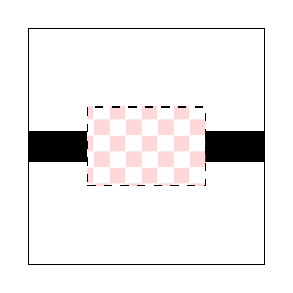
\begin{tikzpicture}
	    \draw[clip] (0,0) rectangle (3,3);
	    \fill[fg] (0,1.3) rectangle (3,1.7);
	    \fill[bg] (0.75,1) -- (2.25,1) -- (2.25,2) -- (0.75,2) -- cycle;
	    \draw[missing] (0.75,1) -- (2.25,1) -- (2.25,2) -- (0.75,2) -- cycle;
        \end{tikzpicture}
    \end{subfigure}%
    \begin{subfigure}[b]{0.33\textwidth}
	\centering
        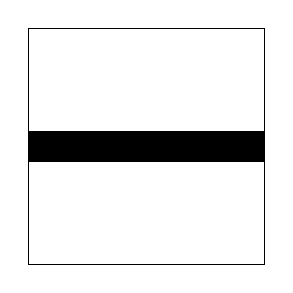
\begin{tikzpicture}
	    \draw[clip] (0,0) rectangle (3,3);
	    \fill[fg] (0,1.3) rectangle (3,1.7);
        \end{tikzpicture}
    \end{subfigure}%
    \begin{subfigure}[b]{0.33\textwidth}
	\centering
        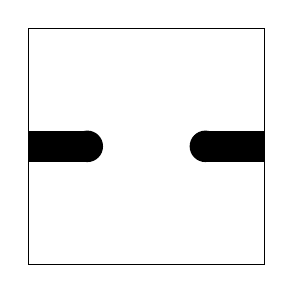
\begin{tikzpicture}
	    \draw[clip] (0,0) rectangle (3,3);
	    \fill[fg] (0,1.3) rectangle (3,1.7);
	    \fill[bg] (0.75,1) -- (2.25,1) -- (2.25,2) -- (0.75,2) -- cycle;
	    \fill[fg] (0.75,1.5) circle[radius=0.2];
	    \fill[fg] (2.25,1.5) circle[radius=0.2];
        \end{tikzpicture}
    \end{subfigure}
    \caption{Krümmungsarme Niveaulinien (mitte) werden bevorzugt}
    \label{fig:inpainting_prefer_non_curved}
\end{figure}

Wir betrachten nun zweidimensionale Bilder $d = 2$.
Anhand von Abbildungen \ref{fig:inpainting_prefer_non_curved} und \ref{fig:inpainting_prefer_non_curved} sieht man, dass in der Regel Bilder bevorzugt werden, bei denen die Kanten (oder Niveaulinien) des Bildes möglichst kurz und gering gekrümmt sind.
Die Niveaulinien eines Bildes stellen auf diese Weise in vielen Fällen eine brauchbare Bewertungsgrundlage dar.
Legt man eine geeignete Bewertung für die Niveaulinien eines Bildes (im Sinne eines Energiefunktionals) fest, so liefert die Summation über alle Höhenlinien eine Bewertung des Gesamtbildes.
Diese Methode wird \emphdef{Levelset-Methode} genannt (siehe Kapitel \ref{chap:image_model}).

Das Bildmodell in dieser Arbeit nutzt die Levelset-Methode und wählt für jede Niveaulinie $\gamma$ die \emphdef{Elastica Energie}
\begin{math}
    \int_{\gamma} \alpha + \beta \kappa^2 \di[s].
\end{math}
Eine Kurve, die diese Energie (unter geeigneten Randbedingungen) minimiert, wird \emphdef{Elastica} genannt.
In der Physik hat sie die Interpretation der Biegeenergie eines elastischen Stabes.
Umfangreiche Herleitungen finden sich in \cite{love1920treatise} und \cite{antman2005problems}, während obige Form der Elastica Energie aus \cite{birkhoff1965nonlinear} stammt.

Die Levelset-Methode liefert uns schließlich für unser Bildmodell (näheres in Kapitel \ref{chap:image_model})
\begin{math}
    \Eimg[u] = \int_{\Omega} \Big(\alpha + \beta (\nabla \cdot \frac{\nabla u}{\nabla u})^2\Big)|\nabla u| \di[x].
\end{math}
Es sei bemerkt, dass dieses geometrische Inpaintingmodell nicht darauf ausgelegt ist wiederkehrende Strukturen zu reproduzieren, die deutlich kleiner als der Inpaintingbereich $D$ sind (siehe Abbildung \ref{fig:inpainting_texture}).
%Wiederkehrende Strukturen außerhalb $D$ werden nicht innerhalb $D$ fortgesetzt.
Hierfür gibt es sogenanntes “texture based inpainting” mit zahlreichen stochastischen Methoden (siehe z.B. \cite{criminisi2004region}).

\begin{figure}[ht]
    \begin{subfigure}[b]{0.33\textwidth}
	\centering
        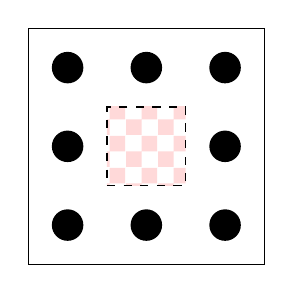
\begin{tikzpicture}
	    \draw[clip] (0,0) rectangle (3,3);
	    \foreach \x in {0.5, 1.5, 2.5}
		\foreach \y in {0.5, 1.5, 2.5}
		    \fill (\x,\y) circle[radius=0.2];
	    \fill[bg] (1,1) -- (2,1) -- (2,2) -- (1,2) -- cycle;
	    \draw[missing] (1,1) -- (2,1) -- (2,2) -- (1,2) -- cycle;
        \end{tikzpicture}
    \end{subfigure}%
    \begin{subfigure}[b]{0.33\textwidth}
	\centering
        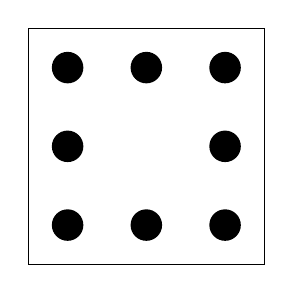
\begin{tikzpicture}
	    \draw[clip] (0,0) rectangle (3,3);
	    \foreach \x in {0.5, 1.5, 2.5}
		\foreach \y in {0.5, 1.5, 2.5}
		    \fill (\x,\y) circle[radius=0.2];
	    \fill[bg] (1,1) -- (2,1) -- (2,2) -- (1,2) -- cycle;
        \end{tikzpicture}
    \end{subfigure}%
    \begin{subfigure}[b]{0.33\textwidth}
	\centering
        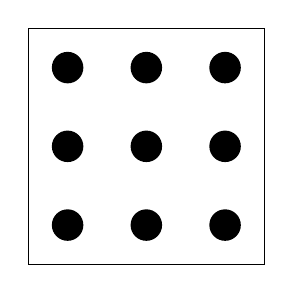
\begin{tikzpicture}
	    \draw[clip] (0,0) rectangle (3,3);
	    \foreach \x in {0.5, 1.5, 2.5}
		\foreach \y in {0.5, 1.5, 2.5}
		    \fill (\x,\y) circle[radius=0.2];
        \end{tikzpicture}
    \end{subfigure}
    \caption{Unser Bildmodell würde das mittlere Bild dem rechten vorziehen}
    \label{fig:inpainting_texture}
\end{figure}


\chapter{Das Euler Elastica Bildmodell} \label{chap:image_model}


\begin{proposition}[Coarea Formel für glatte Bilder] \label{satz:coarea}
    Sei $u \in C^1(\Omega, [0,1])$ und $f \in L^1(\Omega, \R)$.
    Sei $\gamma_\lambda: \R \supset S \to \Omega$ eine stückweise stetige Parametrisierung des Levelsets von $u$ zum Farbwert $\lambda$.
    Dann gilt
    \begin{math}
	\int_0^1 \int_{\gamma_\lambda} f \circ \gamma_\lambda \di[s] \di[\lambda]
	= \int_\Omega f |\nabla u| \di[x]
    \end{math}
    \begin{proof}
        Für einen Beweis, siehe \cite{??}.
    \end{proof}
\end{proposition}



Sei $u \in C^1(\Omega, [0,1])$ ein Bild und $(x_0, y_0) \in \Omega$ mit $\nabla u(x_0, y_0) \neq 0$.
Dann erlaubt $u $



Ein Vorgänger des Euler Elastica Bildmodells ist das sogenannte TV-Bildmodell, welches für ein Bild $u \in C^2(\Omega, [0,1])$ die totale Variation
\begin{math}
    V_\Omega(u) := \int_\Omega |\nabla u| \di[x]
\end{math}
minimiert.






$u \in L^1_{\mathrm{loc}}(\Omega, [0,1])$ die totale Variation
\begin{math}
    V_\Omega(u) := \sup\Set{ \int_\Omega u \div \phi & \phi \in C_0^1(\Omega,\R^d), \|\phi\|_{L^\infty(\Omega)} \le 1}
\end{math}
minimiert.
Man defininiert den Raum der Funktionen mit beschränkter totaler Variation $\BV(\Omega)$ als
\begin{math}
    \BV(\Omega) := \Set{u \in L^1(\Omega, [0,1]) : V_\Omega(u) < \infty}.
\end{math}
Für $u \in C^2$ entspricht dies (siehe \cite[§2.2]{chan2015image})
\begin{math}
    V_\Omega(u) := \int_\Omega |\nabla u| \di[x].
\end{math}






\section{Die Euler Elastica}

\section{Die Level-Set-Methode}
%	Co-Area Formel
%
%	Die Level-Set-Methode
%	\begin{math}
%	    E[u] = \int_{[0,1]} e[\Gamma_\lambda] \di[\lambda]
%	    = \int_{[0,1]} \int_{\Gamma_\Lambda} \alpha + \beta \kappa^2 \di[s] \di[\lambda]
%	\end{math}

\section{Das Euler Elastica Inpainting Modell} % ?

%	\begin{math}
%	    E[u] = \int_{\Omega} (\alpha + \beta \kappa^2) |\nabla u| \di[x]
%	\end{math}
%	für $\kappa = \nabla \cdot (\frac{\nabla u}{|\nabla u|})$.


\chapter{Die “alternating direction” Methode}


\section{Motivation} % komplexität von euler-lagrange und numerische probl.

\section{Augmented Lagrange}

\section{Alternating Direction Method}

%\begin{itemize}
%    \item
%	Operator-Splitting:
%	\begin{math}
%	    &\min_{v,u,m,p,n} \int_{\Omega} (\alpha + \beta(\nabla \cdot n)^2) |p| + \frac{\eta}{2} \int_{\Omega\setminus D} |v - u^0|^2 \\
%	    &\quad\mathrm{s.t.}\quad v = u, p = \nabla u, n = m, |p| = m \cdot p, |m| \le 1.
%	\end{math}
%    \item
%	Augmented Lagrange Funktional:
%	\begin{math}
%	    \scr L[v,u,m,p,n;\lambda_1,\lambda_2,\lambda_3,\lambda_4]
%	    &= \int_{\Omega} (\alpha + \beta(\nabla \cdot n)^2) |p| + \frac{\eta}{2} \int_{\Omega\setminus\Gamma} |v - u^0|^2 \\
%	    &\quad + r_1 \int_\Omega (|p| - m\cdot p) + \int_\Omega \lambda_1 (|p| - m \cdot p) \\
%	    &\quad + \frac{r_2}{2} \int_\Omega |p - \nabla u|^2 + \int_\Omega \lambda_2 \cdot (p - \nabla u) \\
%	    &\quad + \frac{r_3}{2} \int_\Omega (v - u)^2 + \int_\Omega \lambda_3 (v - u) \\
%	    &\quad + \frac{r_4}{2} \int_\Omega |n-m|^2 + \int_\Omega \lambda_4 \cdot (n - m) + \delta_{\ge 1}(m).
%	\end{math}
%    \item
%	Updates:
%	\begin{math}
%	    \lambda_1 &\gets \lambda_1 + r_1 (|p| - m\cdot p), \\
%	    \lambda_2 &\gets \lambda_2 + r_2 (p - \nabla u), \\
%	    \lambda_3 &\gets \lambda_3 + r_3 (v - u), \\
%	    \lambda_4 &\gets \lambda_4 + r_4 (n - m).
%	\end{math}
%\end{itemize}
%
%
%\begin{math}
%    \scr E_1[v]
%    &= \frac{\eta}{2} \int_{\Omega\setminus D} |v - u^0|^2 + \frac{r_3}{2} \int_\Omega (v-u)^2 + \int_\Omega \lambda_3(v - u)\\
%    \scr E_2[u]
%    &= \frac{r_2}{2} \int_\Omega |p - \nabla u|^2 + \int_\Omega \lambda_2 \cdot (p - \nabla u) + \frac{r_3}{2} \int_\Omega (v-u)^2 + \int_\Omega \lambda_3 (v-u) \\
%    \scr E_3[m]
%    &= r_1 \int_\Omega(|p| - m\cdot p) + \int_\Omega \lambda_1 (|p| - m \cdot p) + \frac{r_4}{2} \int_\Omega |n-m|^2 + \int_\Omega \lambda_4 \cdot (n-m) + \delta_{\ge 1}(m) \\
%    &= \frac{r_4}{2} \int_\Omega |x-m|^2 + \delta_{\ge 1}(m) + \const\\
%    \scr E_4[p]
%    &= \int_\Omega (\alpha + \beta(\nabla \cdot n)^2) |p| + r_1 \int_\Omega (|p| - m\cdot p) + \int_\Omega \lambda_1 (|p| - m\cdot p) \\
%    &\qquad + \frac{r_2}{2} \int_\Omega |p - \nabla u|^2 + \int_\Omega \lambda_2 \cdot (p - \nabla u) \\
%    &= \int_\Omega \Big(\alpha + \beta (\nabla \cdot n)^2 + r_1 + \lambda_1\Big) |p| + \frac{r_2}{2} \int_\Omega \Big| p - \big( \nabla u + \frac{r_1 + \lambda_1}{r_2} m - \frac{1}{r_2} \lambda_2 \big) \Big|^2 + \const\\
%    \scr E_5[n]
%    &= \int_\Omega (\alpha + \beta(\nabla \cdot n)^2 ) |p| + \frac{r_4}{2} \int_\Omega |n-m|^2 + \int_\Omega \lambda_4 \cdot (n - m)
%\end{math}
%
%\begin{enumerate}[1)]
%    \item
%	Minimiere
%	\begin{math}
%	    \scr E_1[v]
%	    = \frac{\eta}{2} \int_{\Omega\setminus D} |v - u^0|^2 + \frac{r_3}{2} \int_\Omega (v-u)^2 + \int_\Omega \lambda_3(v - u).
%	\end{math}
%	Variationsrechnung liefert
%	\begin{math}
%	    0 &= \ddx[\eps] \scr E_1[u + \eps \phi] \\
%	    &= \eta \int_{\Omega \setminus D} (v - u^0) \phi + r_3 \int_\Omega (v - u) \phi + \int_\Omega \lambda_3 \phi \\
%	    &= \int_\Omega \Big(\eta (v - u^0)\Ind_{\Omega \setminus D}  + r_3 (v - u) + \lambda_3 \Big) \phi,
%	\end{math}
%	also nach dem Hauptsatz der Variationsrechnung
%	\begin{math}
%	    v = \begin{cases}
%	        u - \frac{\lambda_3}{r_3} & \text{auf $D$}, \\
%		\frac{\eta u^0 + r_3 u - \lambda_3}{\eta + r_3} & \text{auf $\Omega\setminus D$}.
%	    \end{cases}
%	\end{math}
%    \item
%	Minimiere
%	\begin{math}
%	    \scr E_2[u]
%	    = \frac{r_2}{2} \int_\Omega |p - \nabla u|^2 + \int_\Omega \lambda_2 \cdot (p - \nabla u) + \frac{r_3}{2} \int_\Omega (v-u)^2 + \int_\Omega \lambda_3 (v-u).
%	\end{math}
%	Variationsrechnung liefert
%	\begin{math}
%	    0 &= \ddx[\eps] \scr E_2[u + \eps \phi] \\
%	    &= r_2 \int_\Omega (\nabla u - p) \cdot \nabla \phi - \int_\Omega \lambda_2 \cdot \nabla \phi + r_3 \int_\Omega (u - v) \phi - \int_\Omega \lambda_3 \phi \\
%	    &= \int_\Omega (r_2 \nabla u - r_2 p - \lambda_2) \cdot \nabla \phi + \int_\Omega (r_3 u - r_3 v - \lambda_3) \phi,
%	\end{math}
%	als schwache Form einer linearen PDE zweiter Ordnung.
%	%Euler-Lagrange liefert PDE:
%	%\begin{math}
%	%    -r_2 \Laplace u + r_3 u = - r_2 \nabla \cdot p - \nabla \cdot \lambda_2 + r_3 v + \lambda_3.
%	%\end{math}
%    \item
%	Minimiere
%	\begin{math}
%	    \scr E_3[m]
%	    &= r_1 \int_\Omega(|p| - m\cdot p) + \int_\Omega \lambda_1 (|p| - m \cdot p) + \frac{r_4}{2} \int_\Omega |n-m|^2 + \int_\Omega \lambda_4 \cdot (n-m) + \delta_{\ge 1}(m) \\
%	    &= \frac{r_4}{2} \int_\Omega |x-m|^2 + \delta_{\ge 1}(m) + \const,
%	\end{math}
%	wobei $x = \frac{(r_1 + \lambda_1)p + \lambda_4}{r_4} + n$.
%
%	Definiere punktweise
%	\begin{math}
%	    m^* := \begin{cases}
%	        x & \text{für $|x| < 1$}, \\
%		\frac{x}{|x|} & \text{für $|x| \ge 1$}.
%	    \end{cases}
%	\end{math}
%	$m^*$ minimiert $\scr E_3$.
%	Betrachte dazu $\scr E_3[m^* + \phi]$.
%	Wir können ohne Einschränkung fordern, dass $|m^* + \phi| \le 1$ auf $\Omega \setminus N$ für eine Nullmenge $N$, (sonst trivialerweise $\infty = \scr E_3[m^* + \phi] \ge \scr E_3[m^*]$).
%	Setze
%	\begin{math}
%	    M := \Set{x \in \Omega & |x| \ge 1} \setminus N.
%	\end{math}
%	Dann ist auf $M$
%	\begin{math}
%	    1 \ge |m^* + \phi|^2 = \l| \frac{x}{|x|} \r|^2 + 2 \< \frac{x}{|x|}, \phi \> + |\phi|^2,
%	\end{math}
%	also $-2\<\frac{x}{|x|}, \phi\> \ge |\phi|^2$.
%
%	Damit ergibt sich schließlich
%	\begin{math}
%	    \scr E[m^* + \phi]
%	    &= \int_M | \frac{x}{|x|} - x + \phi|^2 \\
%	    &= \int_M | \frac{x}{|x|} - x|^2 + 2 \int_M \<\frac{x}{|x|} - x, \phi\> + \int_M |\phi|^2 \\
%	    &= \scr E[m^*] + \int_M \underbrace{(|x| - 1)}_{\ge 0} \underbrace{(-2\<\frac{x}{|x|}, \phi\>)}_{\ge |\phi|^2} + \|\phi\|_{L^2} \\
%	    &= \scr E[m^*] + \|\phi\|_{L^2}.
%	\end{math}
%	Also ist $m^*$ ein Minimierer von $\scr E_3$ in $L^2$.
%
%	%Explizite Lösung (Lemma):
%	%\begin{math}
%	%    m = \operatorname{proj}_{\le 1}(x)
%	%    = \operatorname{proj}_{\le 1}\Big( \frac{(r_1 + \lambda_1)p + \lambda_4}{r_4} + n \Big)
%	%\end{math}
%    \item
%	Minimiere
%	\begin{math}
%	    \scr E_4[p]
%	    &= \int_\Omega (\alpha + \beta(\nabla \cdot n)^2) |p| + r_1 \int_\Omega (|p| - m\cdot p) + \int_\Omega \lambda_1 (|p| - m\cdot p) \\
%	    &\qquad + \frac{r_2}{2} \int_\Omega |p - \nabla u|^2 + \int_\Omega \lambda_2 \cdot (p - \nabla u) \\
%	    &= \int_\Omega \Big(\alpha + \beta (\nabla \cdot n)^2 + r_1 + \lambda_1\Big) |p| + \frac{r_2}{2} \int_\Omega \Big| p - \big( \nabla u + \frac{r_1 + \lambda_1}{r_2} m - \frac{1}{r_2} \lambda_2 \big) \Big|^2 + \const \\
%	    &= \int_\Omega c |p|_2 + \frac{r_2}{2} \int_\Omega |p - q|^2 + \const
%	\end{math}
%	Es gilt $c, r_2 > 0$ (siehe auch Lagrange-Update für $\lambda_1$).
%	Variationsrechnung liefert für $|p| \neq 0$
%	\begin{math}
%	    0 &= \ddx[\eps] \scr E_4[p + \eps\phi] \\
%	    &= \int_\Omega c \frac{p}{|p|} \cdot \phi + r_2 \int_\Omega (p - q) \cdot \phi.
%	\end{math}
%	Nach dem Hauptsatz der Variationsrechnung
%	\begin{math}
%	    (\frac{c}{|p|} + r_2) p = r_2 q.
%	\end{math}
%	Setze an $p := \lambda q$ mit $\lambda > 0$ also
%	\begin{math}
%	    \lambda = 1 - \frac{c}{r_2 |q|}
%	\end{math}
%	Der Minimierer ist damit gegeben durch
%	\begin{math}
%	    p := \max\Set{0, 1 - \frac{c}{r_2 |q|}} q
%	\end{math}
%	%Explizite Lösung (Lemma: soft thresholding \dots):
%	%\begin{math}
%	%    p = \max\Set{0, 1 - \frac{\alpha + \beta(\nabla \cdot n)^2 + r_1 + \lambda_1}{r_2 |q|}} q
%	%\end{math}
%    \item
%	Minimiere
%	\begin{math}
%	    \scr E_5[n]
%	    &= \int_\Omega (\alpha + \beta(\nabla \cdot n)^2 ) |p| + \frac{r_4}{2} \int_\Omega |n-m|^2 + \int_\Omega \lambda_4 \cdot (n - m)
%	\end{math}
%	Variationsrechnung liefert
%	\begin{math}
%	    0 &= \ddx[\eps] \scr E_5[n + \eps \phi] |_{\eps = 0} \\
%	    &= \int_\Omega 2\beta |p| (\nabla \cdot n) (\nabla \cdot \phi) + \int_\Omega (r_4 n - r_4 m + \lambda_4) \cdot \phi
%	\end{math}
%	%Euler-Lagrange liefert PDE-System:
%	%\begin{math}
%	%    -2 \nabla (\beta |p| \nabla \cdot n) + r_4 (n - m) + \lambda_4 = 0
%	%\end{math}
%\end{enumerate}


\chapter{Numerische Implementierung und Resultate}



\section{Anmerkungen zur Implementierung}
% Finite Elemente, Wahl der Räume, Dune-Zeug

\section{TV-Inpainting}

\section{Euler Elastica Inpainting}

\section{Denoising}


%\begin{itemize}
%    \item
%	Gitterwahl: structured (simplex/kubisch) oder unstructured (simplex, guiding durch Kantendetektor)
%    \item
%	Lineare Lagrange Basis-Funktionen als nahezu einzige Wahl
%    \item
%	Adaptive Strategien (z.B. refine/coarse gemäß $n = \nabla u$), Vergleich
%    \item
%	Parameter-Tweaking ($\alpha$, $\beta$, $\eta$, $r_1, r_2, r_3, r_4$) und -Interpretation
%    \item
%	Startwert-Tweaking ($v, u, m, p, n, \lambda_1, \lambda_2, \lambda_3, \lambda_4$)
%\end{itemize}

%\section{Weitere Anwendungen}
%
%\begin{itemize}
%    \item
%	Debluring
%    \item
%	Upscaling
%\end{itemize}


%\section{Appendix}
%
%\subsection{Co-Area-Formel}
%\subsection{Euler-Lagrange}
%\subsection{Soft-Thresholding?}

\bibliographystyle{plain}
\bibliography{thesis}

\end{document}

